\documentclass[12pt]{article}
\usepackage{graphicx}
\usepackage[utf8]{inputenc}
\usepackage{makecell}
\usepackage[margin=1in]{geometry}
\usepackage[T1]{fontenc}
\usepackage{mathptmx}
\usepackage[normalem]{ulem}
\usepackage{csquotes}
\graphicspath{ {./media/} }
\renewcommand\theadalign{bc}
\renewcommand\theadfont{\bfseries}
\renewcommand\theadgape{\Gape[4pt]}
\renewcommand\cellgape{\Gape[4pt]}

\usepackage[
backend=biber,
style=numeric,
sorting=none,
citestyle=ieee
]{biblatex}

\addbibresource{references.bib}

%opening
\title{Software Requirement Specification Document for CSE334 Course Project}
\author{
Abdelrahman Mohamed, Maeen Mohamed, Omar El Nahass, \\Omar Ashraf, Roaa Mohamed\\
Supervised by: Dr. Essam Eliwa, Eng. Omar Magdy
}
\usepackage{hyperref}
\hypersetup{
colorlinks=true,
linkcolor=black,
urlcolor=blue,
}

\begin{document}
\maketitle

\begin{table}[htp]
\caption{Document version history}
\begin{center}
\begin{tabular}{|c|c|l|}
\hline
\thead{Version}    & \thead{Date} & \thead{Reason for Change}  \\ \hline
1.0 & 17-Apr-2023   & \makecell[l]{SRS First version’s specifications are defined.}   \\ \hline
%1.1 & 2-Dec-2022   & \makecell[l]{....\\.....\\........} \\ \hline
%1.3 & 10-Dec-2022   & \makecell[l]{......\\......} \\ \hline
\end{tabular}
\end{center}
\end{table}

\begin{table}[htp]
\begin{tabular}{cc}
\thead{Project:}    & {Shoezone Store Website}  
\end{tabular}
\end{table}

\begin{table}[htp]
\begin{tabular}{cc}
\thead{GitHub:}  \url{http://github.com/omarafal/se-majortask.git}
\end{tabular}
\end{table}


\pagebreak
\tableofcontents
\pagebreak
\begin{abstract}
In the last few years, online shopping has become an integral part of our daily lives especially after the COVID-19 pandemic. Obtaining a web application is almost mandatory for any shop that aims to reach a wider range of audiences. Our Project is aimed to create a full website for a small business selling different types of shoes (men and women) that has a sleek modern design with user-friendly options. We plan to apply an incremental development process as we want to involve the customer as much as possible and regularly update the application based on said customer's changing requirements.
With a team of sophomore students boasting extensive knowledge in the field, we are well-placed to help our clients grow and thrive - even in challenging times. By really getting to know our customers, our talented team can offer unique and customized solutions backed by data-driven analysis and broad research.
As a team, we believe in building long-lasting client partnerships which help us all grow. Our main goal is to create unique websites that attract a bunch of users from all over the world.

\end{abstract}


\section{Introduction}
\subsection{Purpose of this document}
The Software Requirement Specification Document (SRS) of this project is to overview and outline the requirements of the Shoezone Website. The intended audiences of the external stakeholder type are Dr. Essam Eliwa, Eng. Omar Magdy and the website's owner while of the internal stakeholder type are the end-users. Shoezone Website eases ordering for all Shoezone store clients of different ages and knowledge about websites; The website allows the user to order using any internet browser as the website will account for the different browsers the users might use to access the website.
\subsection{Scope of this document}
The SRS document of this project shall include the following
\begin{itemize}
\item Already delivered: front-end, proposal document.
\item Yet to be delivered: back-end, testing document, and SDD document.
\item A guideline for the project's expected schedule.
\item A list of functional and non-functional requirements.
\end{itemize}



%\subsection{Business Context}
%200 word Limit


\section{Similar Systems}
\subsection{Academic}
According to Adaptation of usability principles in responsive web design technique for e-commerce development \cite{majid2015adaptation}:\\
Interface web development is based on usability, easy to be user friendly, effective and efficient. Responsive web design is becoming more important due to high demand for user friendly interfaces. This paper aimed to analyse the most appropriate usability principles in responsive web design. The results revealed five usability principles: consistency, familiarity, flexibility, efficient feedback and aesthetically pleasing. These principles help to provide a website with greater look, consistent and tailored according to different devices.\\
According to Implementing responsive web design for enhanced web presence \cite{mohorovivcic2013implementing}:\\
The mere act of appearing online and being found by multiple search engines, however, is no longer sufficient.\\
Websites must be optimised for all devices in order to offer the optimal user experience since increasingly people are using smartphones and tablets in addition to desktop computers and notebooks to access the Internet.\\
Responsive web design should allow a website to adjust to any of these devices, i.e., their resolutions.


\subsection{Business Applications}
Similar business applications:
\begin{itemize}

\item
Charles and Keith: A store that sells multiple products including shoes.
 \begin{figure}[h]
\centering
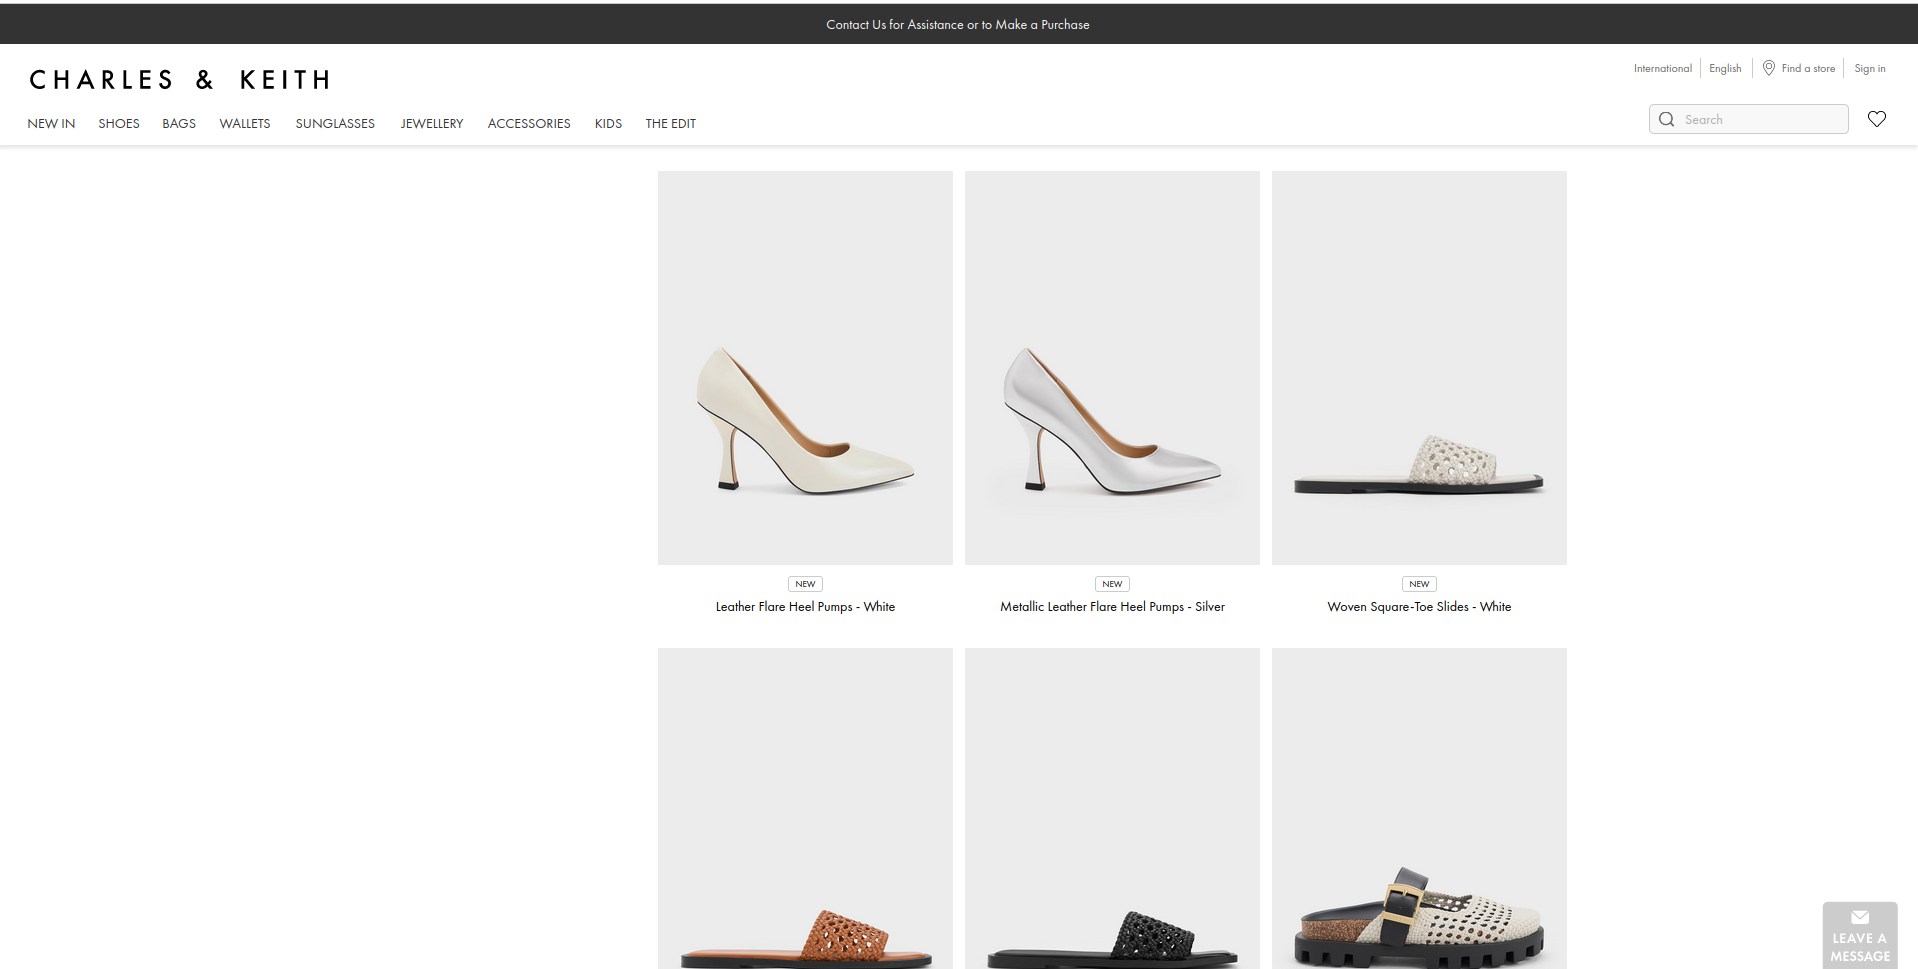
\includegraphics[width=0.8\linewidth]{chK.png}
\caption{Charles and Keith's website}
\end{figure}
\end{itemize}
\newpage
\begin{itemize}
\item 
Adidas: A famous brand that sells different types of shoes.
 \begin{figure}[h]
\centering
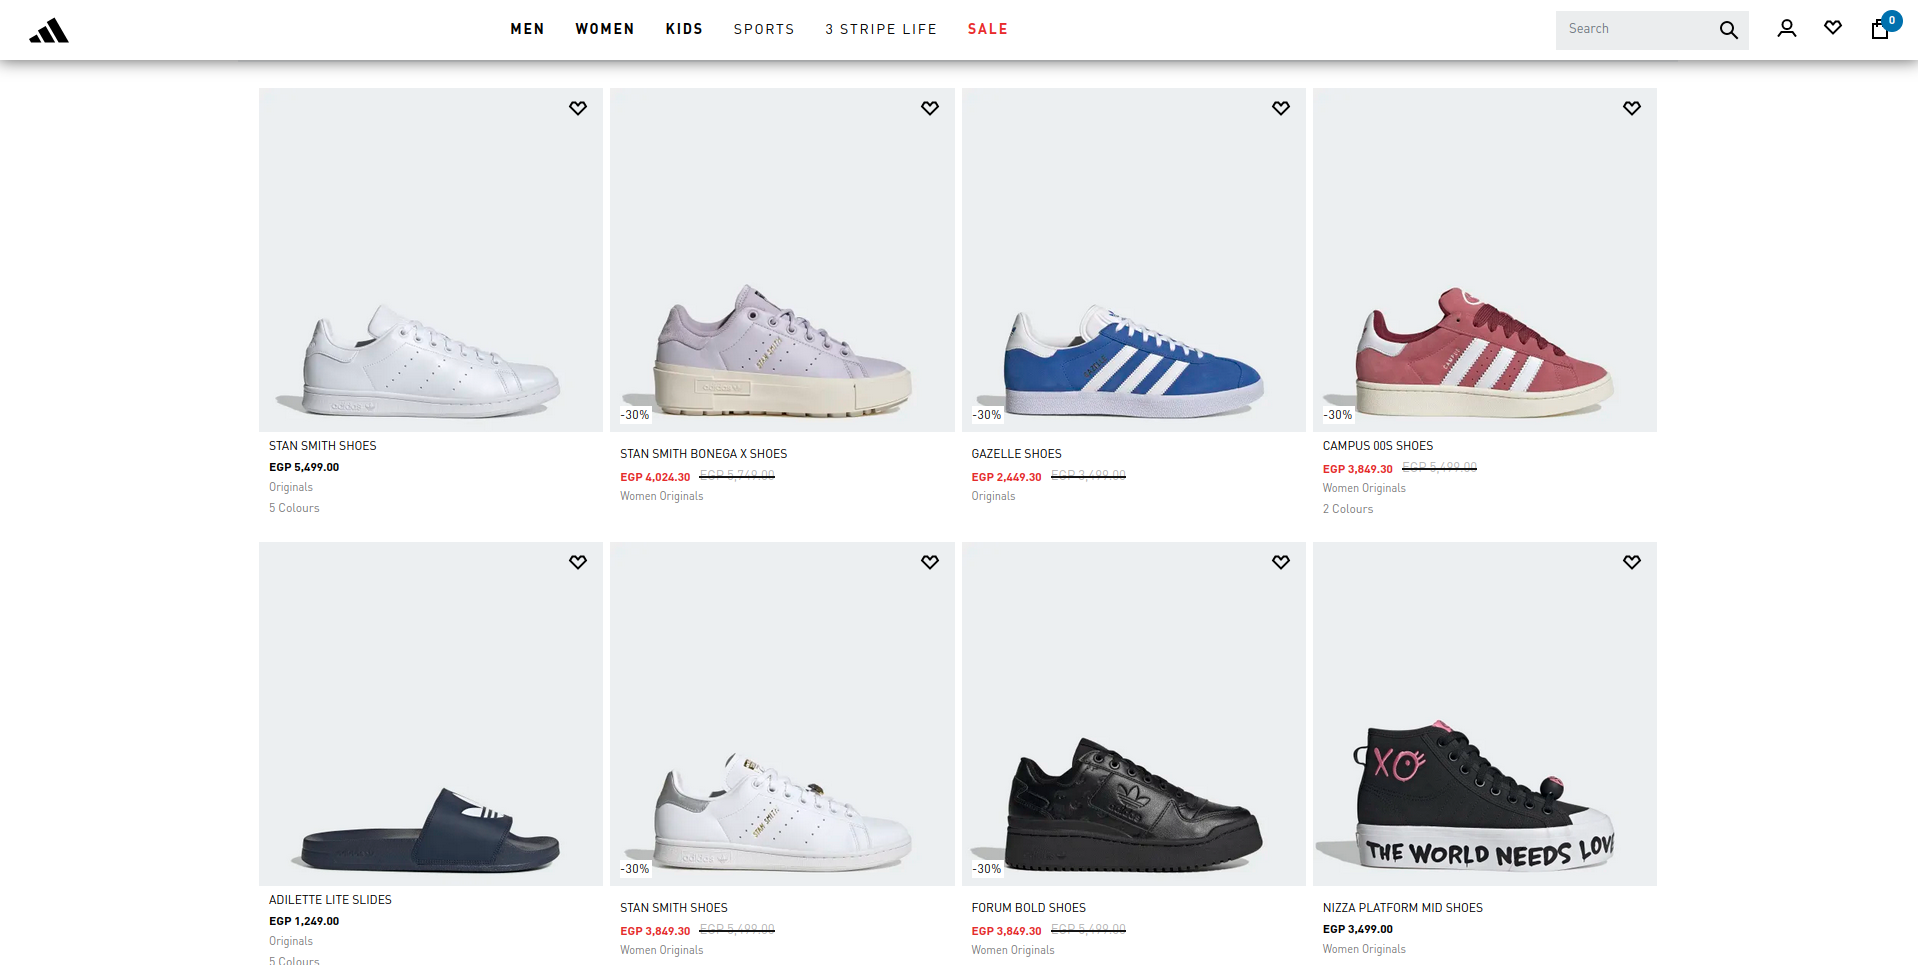
\includegraphics[width=0.8\linewidth]{adidas.png}
\caption{Adidas' website}
\end{figure}

\end{itemize}

\section{System Description}

\subsection{Problem Statement}
Visiting physical stores with the uncertainty of finding a suitable pair of shoes can be quite time-wasting as well as exhausting. Designing and developing a user-friendly web application can be quite a challenge. Nowadays, website developers are challenged on implementing the website before a competitor can issue his website, therefore the satisfaction of the users of e-commerce websites decreased, as most of the developers do not consider some obstacles that meet the user, for example, according to the American Management Association Survey in 1997, slow response time, lack of user-friendliness, and poor website design. Furthermore, the clients are sometimes distracted by the website’s actions as the website does not give feedback for their actions.

Our goal is to design a website that minimizes the number of clicks through which the user will reach the page he wants. This is by locating the important data in the most places the users usually look at when they first open the website, for instance, in the upper left corner of the page or the upper part of the page generally, also we intend on keeping the least important information at the bottom of the page, so it does not distract the user. In addition, we will consider designing a website that responds to the user’s interaction with the website.


\subsection{System Overview}
Shoezone Website displays the available shoe in store for two categories, men and women. It contains separate pages for said categories to ease the search; In addition to, having a search bar on the home page to aid in finding a specific item. Shoezone Website also provides online ordering; Therefore, there is a cart page to which all the items to be ordered are added, so the client can directly go from it to the checkout page to complete his order.

\subsection{System Scope}
The website is built to:
\begin{itemize}
 \item Allow users to create accounts.
 \item Display all the available shoes with their available sizes and colors.
 %\item Allow the clients to order through any available shoes. <---- Written by Roaa
 \item Enable the logged-in user to add any shoe to his cart.
 \item Inform the client of the estimated delivery time.
 \item Provide different types of payment like Cash, Visa, Master Card, and Meeza.   
 \item Not save any sensitive information like credit card details.
\end{itemize}
\subsection{System Context}
 \begin{figure}[h]
\centering
\includegraphics[width=0.8\linewidth]{context.png}
%\caption{Adidas' website}
\end{figure}
%\newpage
\subsection{Objectives}
\begin{itemize}
 \item Creating an eye appealing, user-friendly website.
 \item Obtaining a wide of range of shoes to be available to users online.
 \item Not repulsing users by having a fast response time.
 \item The users can access the store whenever they want from the comfort of their home.
 \item The design is privileged with clear navigation to help the clients with their orders.
\end{itemize}

\subsection{ User Characteristics}
Internal stakeholders are those within a company whose interest stems from direct employment, ownership or investment.
\begin{itemize}
\item Dr. Essam Eliwa: Project supervisor
\item Eng. Omar Magdy: Project supervisor
\item Application Owner: Owners of Shoezone shall not require an extensive knowledge of web development nor database handling as there will be an admin user interface available for them to easily add or edit or delete shoes.
\item Project team: Designers and developers of the Shoezone web application.
%\item Owners: It is required from the owners to have minimum knowledge of database handling, as we are using Django, which already provides an admin user interface which enables them to.
\end{itemize}
External stakeholders are those who do not directly work with a company but are affected somehow by the actions and outcomes of the business.
\begin{itemize}
\item Customers: Individuals who are not expected to comprehend a lot about computers or web development; the only skill needed is to be capable of using computer software.
\item Government
\item Shoe supplier: A supply outlet that provides products to Shoezone
\end{itemize}

\pagebreak 
\section{Functional Requirements}
\subsection{System Functions}\label{System Functions}
\includegraphics[width=1\linewidth]{functions.png}
\subsubsection{Admin}
The admin should be able to:
\begin{itemize}
\item Add shoe.
\item Remove shoe.
\item Edit shoe details including size, color, and prices
\item Monitor users.
\begin{itemize}
    \item Add users.
    \item Remove users.
    \item Edit user's details.
\end{itemize}
\item View cart items for individual users.
\item Keep track of clients orders status.
\end{itemize}
\subsubsection{Client}
The Customer should be able to:
\begin{itemize}
\item Sign up to create an account with personal emails and custom usernames.
\item Directly sign in, if he/she has an existing account.
\item Search for a shoe through the search bar.
\item View shoe details.
\item Select wanted qualities for shoes before adding to cart (color and size).
\item Add and remove shoes from the cart.
\item Edit personal details including first name, last name, and email through profile page.
\item Change account's password.
\end{itemize}
\section{Design Constraints}
Shoezone website helps store customers view and order any shoes they want from their homes through a user-friendly website that is hosted online on pythonanywhere using a 'Beginner' account therefore there tend to be a few limitations. 

\subsection{ Standards Compliance}
A working internet connection and almost any browser.

\subsection{ Hardware Limitations}
\begin{itemize}
    \item A CPU allowance of 100 seconds only.
    \item A limited/low bandwidth
    \item A private file storage of merely 512 MB.
\end{itemize}

\section{Non-functional Requirements}
\begin{itemize}
\item The web application shall have at least 5 GB of space available to use to store images and any other important media.
\item Upgrade Django's default database from SQLite to MySQL to ensure the web application can handle a higher load of traffic, significantly more than 100K hits/day.
\item The website must be checked upon ever three months to make sure it still works on pythonanywhere.
\item The login/register systems must hash the passwords for increased security.
\item An ease of access to the web application must be provided and supporting multiple browsers, at least 90\% of them, is important by testing the web application on different browsers and adjusting it accordingly.
\item The website shall be easy to use.
\item The website should be designed in a way that it only takes a user around three minutes to be fully capable of navigating through it.

\end{itemize}

% \section{Data Design}
% Data Description (200 word Limit)


% \section{Preliminary Object-Oriented Domain Analysis}
% Initial Class Diagram


\section{Operational Scenarios}
\textbf{Initial Assumption}: The user logs in or registers on the site. Tries searching for a shoe and adds it to cart.\\
\textbf{Normal}: The customer views the shoes on the website. If the customer decides to order any of the shoes, it will require him to sign up if it is his first time using the website or sign in using his account if the customer has one. Subsequently, he will add any shoes he wants to the cart to
checkout and place the order.\\
\textbf{What can go wrong}:
\begin{itemize}
\item The user signs up with an existing email.
\item The user enters a wrong password while trying to signing in.
\item The user tries resetting the password and in doing so enters his old password.
\item The user enters incorrect credit card details while trying to complete a purchase.
\end{itemize}
\textbf{System state on completion}: The user should be capable of viewing and searching for shoes before signing up or signing in if the user wanted to place an order then he should sign up or sign in and proceed to checkout providing his credit card credentials, that don't get saved, and completes the purchase.
\section{Project Plan}
\includegraphics[width=1\linewidth]{media/timeplan.png}

\section{Appendices}

\subsection{Definitions, Acronyms, Abbreviations}
COVID-19: Coronavirus disease of 2019. \\
SDD Document: Software Design Document. \\
pythonanywhere: Online integrated development environment and web hosting service based on the Python programming language.\\
SQLite: Database engine. \\ 
MySQL: Open-source relational database management system. \\

\printbibliography
\end{document}